\documentclass{article}
\usepackage{listings}

% Language setting
% Replace `english' with e.g. `spanish' to change the document language
\usepackage[english]{babel}

% Set page size and margins
% Replace `letterpaper' with`a4paper' for UK/EU standard size
\usepackage[letterpaper,top=2cm,bottom=2cm,left=3cm,right=3cm,marginparwidth=1.75cm]{geometry}

% Useful packages
\usepackage{amsmath}
\usepackage{graphicx}
\usepackage[colorlinks=true, allcolors=blue]{hyperref}

\title{Assignment 1}
\author{Owen Bean}

\begin{document}
\maketitle

\section{Code}

The code is located on \href{https://github.com/owenbean400/assignment1COS470}{https://github.com/owenbean400/assignment1COS470}. The programs is under the code folder with the name Question with the number that the question the code was for.

\section{Question 1 Response - Zipf's law}

Examining the graph below of the words versus probability of Questions in comparison to the ideal Zipf's law, both graph lines are concave and decreasing. The difference between the two is that Zipf's law is decreasing at a faster rate than the words in Questions. Considering the small sample size of 171 words, the Question line characteristics is similar to Zipf's law. Therefore, I conclude that the Questions follow the expectations of Zipf's law.

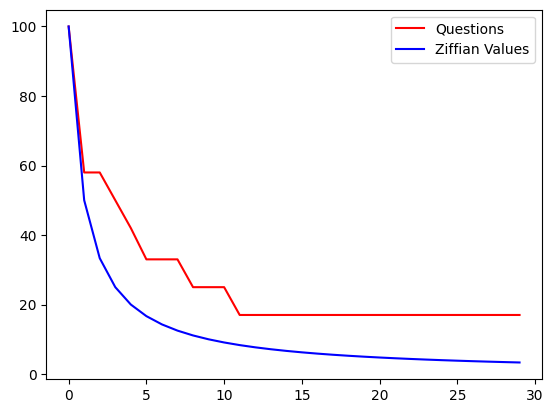
\includegraphics[width=400]{images/zipf.png}

\section{Question 2 Response - Word Cloud}

The most common word, including stop words, is "the". "The" is the most popular English word. Upon examination of the word cloud sans stop words, "word" is the most frequent word. "Word" on the word cloud including stop words appears to be approximately 50\% of the frequency of "the". This indicates that there is a significant number of stop words that are more frequent than "word". Finally, approximately half of the top 20 words were stop words. \\

wordCloud with stop words: \hspace*{1.6in} wordCloud without stop words:

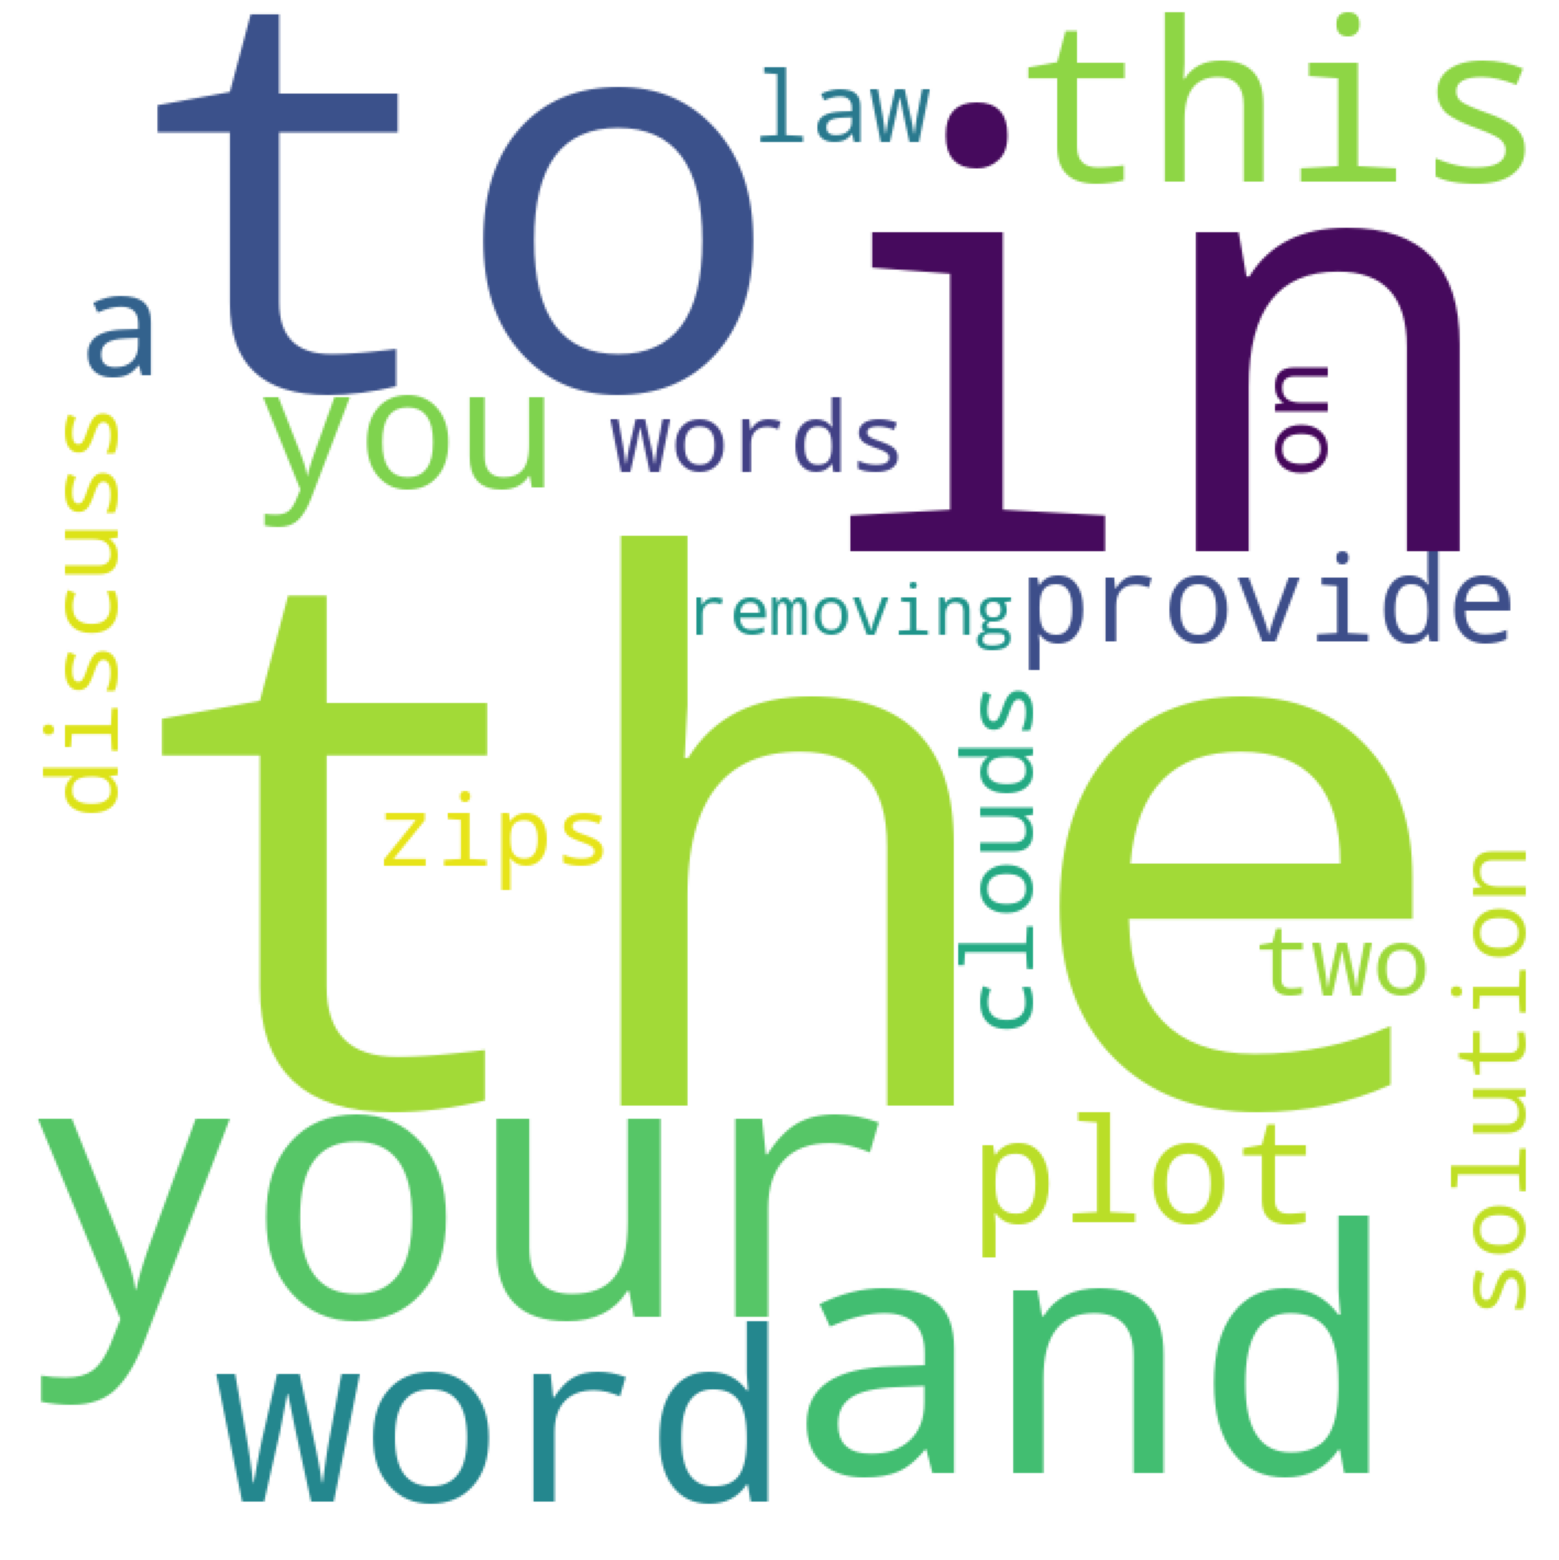
\includegraphics[width=200]{images/wordCloud.png}
\hspace*{0.5in}
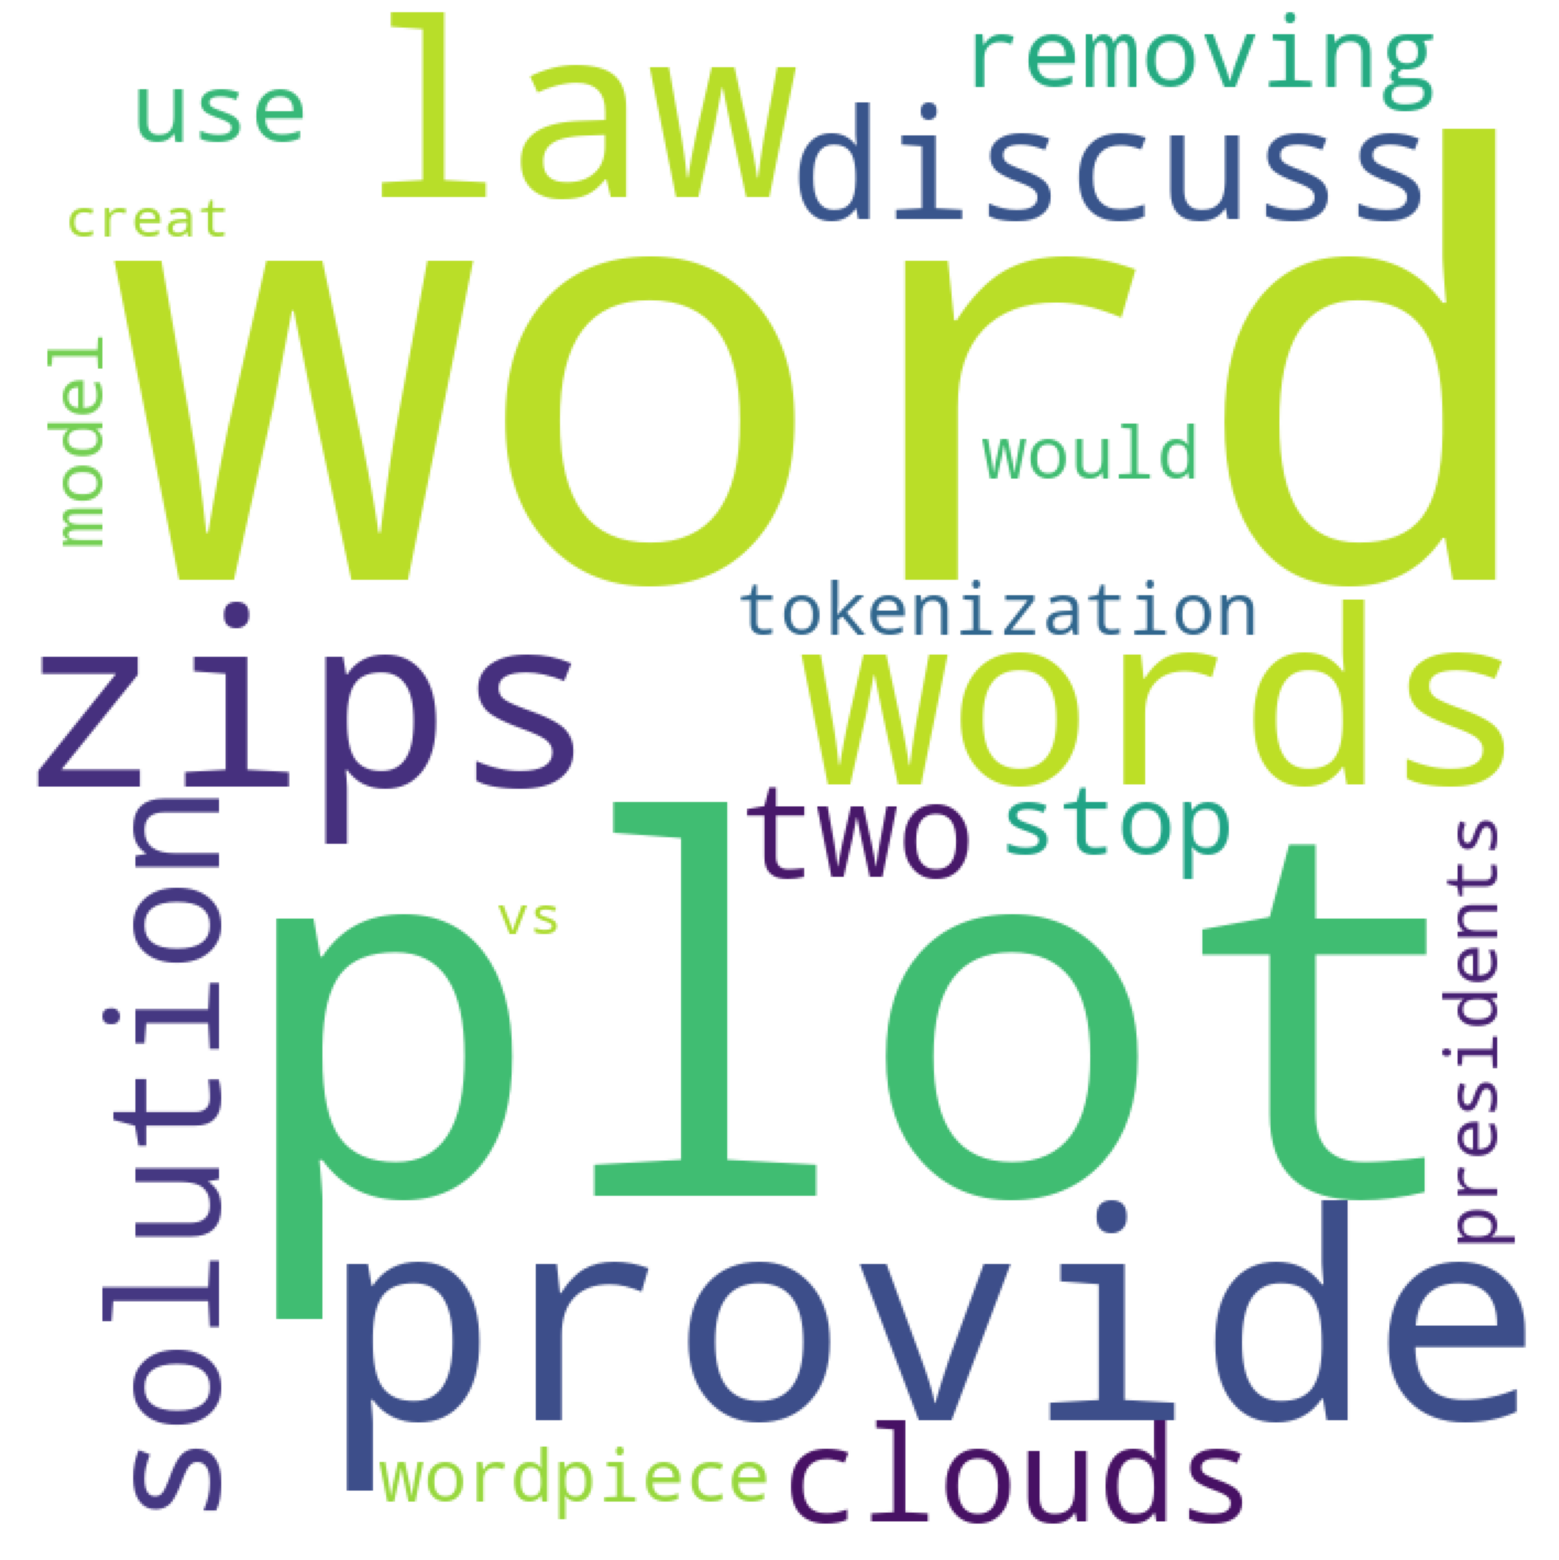
\includegraphics[width=200]{images/wordCloudNoStopWords.png}

\section{Question 3 - Find president's speech}

In order to ascertain the likelihood of a speech being uttered by a president, I would procure all of the speeches given by a president. I would then divide all of the speeches into three segments, with 50\% of the speeches designated to the training set, 25\% for validating the training model, and the remaining 25\% for testing the training model. I would train the model with a bigram model on the 50\% of speeches, as presidents likely use a combination of words in unison, leaving the rest of the speeches for testing. Subsequently, 25\% of the speeches would be used to validate that the model is functioning as intended. Finally, I would combine the 25\% of speeches saved for testing with random other speeches in order to evaluate whether the model can differentiate between a president's speech and a non-president's speech.

\section{Question 4 - Word Piece}

The BPE and WordPiece are equivalent when it comes to splitting words into characters. Despite being divided into characters, the BPE will merge the most frequent pairs, while WordPiece will merge based on the largest combination yielding a frequency of pair divided by the frequency of the first element multiplied by the frequency of the second element.

For "low low low low low lowest lowest newer newer newer newer newer newer wider wider wider new new" the characters will split up as {['\#\#d', '\#\#e', '\#\#i', '\#\#o', '\#\#r', '\#\#s', '\#\#t', '\#\#w', 'l', 'n', 'w']}. The \#\# is a place holder that a character was in front of that token. When doing the (frequency of pair) / (frequency of first element * frequency of second element) will yield:

\begin{verbatim}
    ('l', '##o'): 0.14285714285714285
    ('##o', '##w'): 0.06666666666666667
    ('##w', '##e'): 0.028070175438596492
    ('##e', '##s'): 0.05263157894736842
    ('##s', '##t'): 0.5
    ('n', '##e'): 0.05263157894736842
\end{verbatim}

Because ('\#\#s', '\#\#t') is the highest score, that gets added to the vocabulary. {['\#\#d', '\#\#e', '\#\#i', '\#\#o', '\#\#r', '\#\#s', '\#\#t', '\#\#w', 'l', 'n', 'w', '\#\#st']}. Doing this until the vocabulary size is 20 will yield {['\#\#d', '\#\#e', '\#\#i', '\#\#o', '\#\#r', '\#\#s', '\#\#t', '\#\#w', 'l', 'n', 'w', '\#\#st', 'wi', 'wid', 'lo', 'low', '\#\#est', 'lowest', 'ne', 'new']}. 

\begin{verbatim}
    Input: newer -> Tokens: new, ##e, ##r     n -> ne -> new, \#\#e, \#\#r
    Input: lower -> Tokens: low, ##e, ##r     l -> lo -> low, \#\#e, \#\#r
\end{verbatim}

That tokenization is different compared to BPE, which would yield ("newer") and ("low", "er").

\end{document}